\documentclass[11pt,a4paper]{article}
\usepackage[margin=2.2cm]{geometry}
\usepackage{fontspec}
\usepackage{amsmath,amssymb}
\usepackage{graphicx,booktabs,xcolor,enumitem,microtype}
\usepackage[section]{placeins}
\usepackage[most]{tcolorbox}
\usepackage{tikz}
\usetikzlibrary{arrows.meta,positioning,decorations.pathmorphing}
\usepackage[colorlinks=true,linkcolor=blue!50!black,urlcolor=blue!50!black]{hyperref}
\setmainfont{texgyrepagella}[Extension=.otf,UprightFont=*-regular,BoldFont=*-bold,ItalicFont=*-italic,BoldItalicFont=*-bolditalic]
\setsansfont{texgyreheros}[Extension=.otf,UprightFont=*-regular,BoldFont=*-bold,ItalicFont=*-italic,BoldItalicFont=*-bolditalic]
\graphicspath{{figures/}{figures_quick/}}
\setlength{\parskip}{0.5em}\setlength{\parindent}{0pt}

% ---------- boxes
\newtcolorbox{idea}[1][]{colback=blue!4,colframe=blue!50!black,fonttitle=\bfseries\sffamily,title={Key idea#1},sharp corners=south,boxrule=0.6pt}
\newtcolorbox{tryit}[1][]{colback=green!5,colframe=green!40!black,fonttitle=\bfseries\sffamily,title={Try it#1},sharp corners=south,boxrule=0.6pt}
\newtcolorbox{think}[1][]{colback=orange!6,colframe=orange!70!black,fonttitle=\bfseries\sffamily,title={Think about it#1},sharp corners=south,boxrule=0.6pt}
\newtcolorbox{control}[1][]{colback=violet!5,colframe=violet!60!black,fonttitle=\bfseries\sffamily,title={Control corner#1},sharp corners=south,boxrule=0.6pt}
\newcommand{\btn}[1]{\tikz[baseline=(b.base)]\node[draw,rounded corners=2pt,fill=gray!15,inner sep=2pt,font=\sffamily\footnotesize](b){#1};}
\newcommand{\param}[1]{\texttt{\small #1}}

\title{\sffamily\bfseries Predators, Prey and Feedback\\[0.3em]
\large A hands-on guide to dynamic systems with the Lotka ecosystem simulator\\[0.3em]
\normalsize\mdseries For first-year Systems \& Control students}
\author{Hugo Macedo, with Hermes Agent \& Claude}
\date{}

\begin{document}
\maketitle
\thispagestyle{empty}

\begin{center}
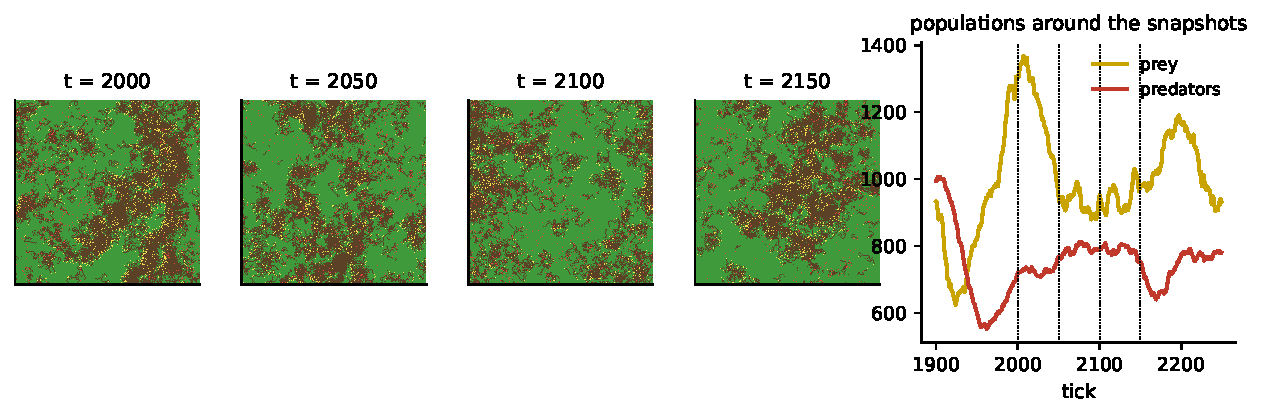
\includegraphics[width=0.95\linewidth]{snapshots.pdf}
\end{center}

\vspace{-0.5em}
\begin{idea}[: what this guide is about]
A \emph{dynamic system} is anything whose future depends on its present: a cruise-controlled car, a
thermostat-heated room, a bank balance, an epidemic\ldots\ and an ecosystem. In this guide you will
\emph{play} with a simulated ecosystem of vegetation, prey and predators, and use it to discover, one by one,
the ideas that the rest of your Systems \& Control course is built on: \textbf{state, feedback,
equilibrium, stability, oscillation, delay, nonlinearity, models} and finally \textbf{control}.
Very little mathematics is needed; curiosity and the simulator are enough.
\end{idea}

\tableofcontents
\newpage

%=====================================================================
\section{Getting started}
%=====================================================================
You need the two browser pages of the Lotka project (your instructor will give you the address, usually
\url{http://127.0.0.1:8765}):

\begin{itemize}[nosep]
  \item \textbf{Simulator} (\texttt{/}): the grid of coloured pixels, live charts and all the knobs.
  \item \textbf{Command Center} (\texttt{/evolve}): lets the computer search for parameter sets by itself (Section~\ref{sec:opt}).
\end{itemize}

\textbf{Reading the grid.} Every pixel is a patch of land. \textcolor{green!50!black}{\textbf{Green}} =
vegetation, \textcolor{brown}{\textbf{brown}} = bare soil that is regrowing,
\textcolor{yellow!70!black}{\textbf{yellow}} = a prey animal, \textcolor{red!70!black}{\textbf{red}} = a
predator. The world wraps around: leaving on the right brings you back on the left.

\textbf{The rules} (one \emph{tick} = one time step):
\begin{enumerate}[nosep]
  \item Eaten vegetation grows back after \param{veg\_regrow\_time} ticks.
  \item Animals move one cell. Prey drift towards grass and away from predators; predators drift towards prey.
  \item A prey next to a predator is eaten (a predator eats at most one per tick by default).
  \item Prey eat the grass under and around them. A prey that goes \param{prey\_starve\_time} ticks without
        enough food dies; a predator dies after \param{predator\_starve\_time} ticks without a meal.
  \item Fed animals may have one offspring in a free neighbouring cell.
\end{enumerate}

\textbf{The controls.} \btn{Play}/\btn{Step} run time forward; \btn{Apply \& reset} restarts with the
parameters on the left; the \textbf{Preset} menu loads ready-made scenarios; the \textbf{Shock} buttons
suddenly remove or add animals; the charts on the right show populations over time, the \emph{phase portrait}
(prey vs predators) and births/deaths per tick. The panel at the bottom compares the simulation with
mathematical models (Section~\ref{sec:models}).

\begin{tryit}[: first contact]
Load the preset \emph{Stable coexistence} and press \btn{Play}. Watch the grid for a minute.
Then press \btn{Pause} and use \btn{Step} a few times. Write down three things you notice.
\end{tryit}

%=====================================================================
\section{What is a dynamic system?}
%=====================================================================
\begin{idea}[: state]
The \textbf{state} of a system is the information you need \emph{now} to work out what happens \emph{next}.
A rule (here: the five rules above) takes the state at tick $t$ and produces the state at tick $t+1$:
\[ \text{state}(t+1) = \text{rule}\big(\text{state}(t),\ \text{inputs}(t)\big). \]
\end{idea}

For our ecosystem the \emph{true} state is enormous: the content of every cell, plus every animal's hunger and
age --- more than a hundred thousand numbers. Engineers almost never work with the full state. Instead we pick a
few \textbf{state variables} that summarise it well: the number of prey $x$, the number of predators $y$ and
the amount of vegetation $v$. The charts show exactly these three numbers.

An \textbf{input} is something we can push on from outside (later: harvesting), an \textbf{output} is what we
measure (the counts in the cards at the top), and a \textbf{disturbance} is a push we do not control
(the Shock buttons will play that role).

\begin{think}
Is the population of prey next tick fully decided by today's population of prey? Why do you also need to know
how many predators there are? What about vegetation? This is why a dynamic system usually needs
\emph{several} state variables.
\end{think}

%=====================================================================
\section{Feedback loops}
%=====================================================================
Look at how the three variables influence each other (Fig.~\ref{fig:loops}). An arrow marked $+$ means
``more of A leads to more of B''; $-$ means ``more of A leads to less of B''.

\begin{figure}[!htb]
\centering
% Shared TikZ figure: causal-loop diagram of the ecosystem (used by paper and guide)
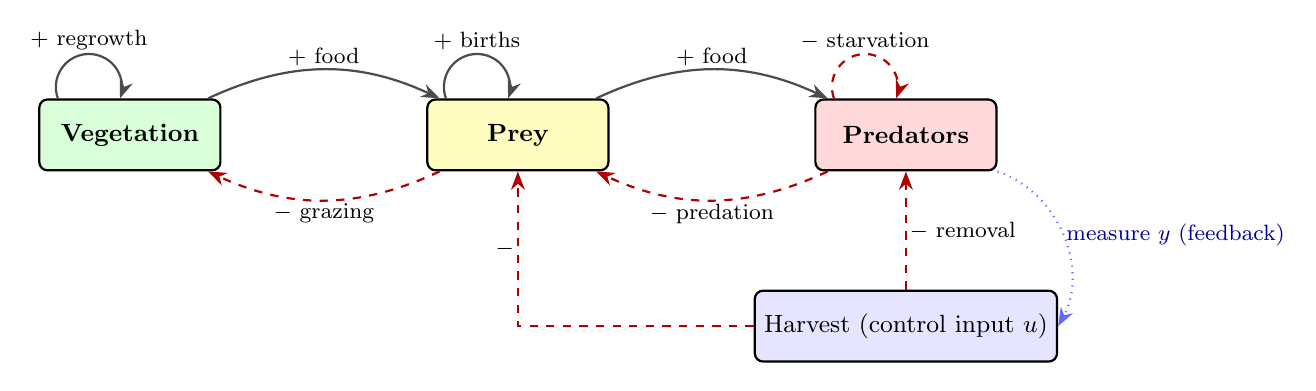
\begin{tikzpicture}[
  node distance=2.6cm, >=Stealth,
  stock/.style={draw, rounded corners=3pt, minimum width=2.3cm, minimum height=0.9cm, font=\small\bfseries, thick},
  lbl/.style={font=\footnotesize, inner sep=1pt},
  plusarrow/.style={->, thick, draw=black!70},
  minusarrow/.style={->, thick, draw=red!70!black, dashed}]
  \node[stock, fill=green!15]  (V) {Vegetation};
  \node[stock, fill=yellow!25, right=of V] (X) {Prey};
  \node[stock, fill=red!15, right=of X] (Y) {Predators};
  \node[stock, fill=blue!10, below=1.5cm of Y, font=\small] (H) {Harvest (control input $u$)};
  % food chain
  \draw[plusarrow] (V) to[bend left=25] node[lbl, above] {$+$ food} (X);
  \draw[minusarrow] (X) to[bend left=25] node[lbl, below] {$-$ grazing} (V);
  \draw[plusarrow] (X) to[bend left=25] node[lbl, above] {$+$ food} (Y);
  \draw[minusarrow] (Y) to[bend left=25] node[lbl, below] {$-$ predation} (X);
  % self loops
  \draw[plusarrow] (X.north west) ++(0.25,0) arc[start angle=200, end angle=-20, radius=0.42] node[lbl, pos=0.5, above] {$+$ births};
  \draw[plusarrow] (V.north west) ++(0.25,0) arc[start angle=200, end angle=-20, radius=0.42] node[lbl, pos=0.5, above] {$+$ regrowth};
  \draw[minusarrow] (Y.north west) ++(0.25,0) arc[start angle=200, end angle=-20, radius=0.42] node[lbl, pos=0.5, above] {$-$ starvation};
  \draw[minusarrow] (H) -- node[lbl, right] {$-$ removal} (Y);
  \draw[minusarrow] (H.west) -| node[lbl, pos=0.75, left] {$-$} (X.south);
  \draw[->, thin, draw=blue!60, dotted, thick] (Y.south east) to[bend left=50] node[lbl, right, text=blue!60!black] {measure $y$ (feedback)} (H.east);
\end{tikzpicture}

\caption{Causal-loop diagram of the ecosystem. Solid arrows reinforce ($+$), dashed arrows oppose ($-$).
The harvest box is the control input used in Section~\ref{sec:control}.}
\label{fig:loops}
\end{figure}

\begin{idea}[: two kinds of loop]
\textbf{Reinforcing (positive) loops} amplify change: more prey $\rightarrow$ more births $\rightarrow$ even more prey.
On their own they give explosive growth.\\
\textbf{Balancing (negative) loops} oppose change: more prey $\rightarrow$ more predators $\rightarrow$ fewer prey.
They push the system back. Follow the loop prey $\rightarrow$ predators $\rightarrow$ prey: one $+$ and one $-$, so the
overall sign is $-$: it is balancing.
\end{idea}

\begin{tryit}[: break a loop]
Load \emph{Predator starvation}: predators die after only 3 hungry ticks, so the predation loop is cut almost
immediately. What happens to the prey? What limits them now? (Hint: look at the green.)
Then load \emph{Prey overpopulation} (no predators at all, fast breeding). Describe what the reinforcing birth
loop does at first and which balancing loop eventually stops it.
\end{tryit}

%=====================================================================
\section{Equilibrium}
%=====================================================================
\begin{idea}[: equilibrium]
An \textbf{equilibrium} is a state that does not change on its own: everything that flows in is balanced by
what flows out. For a population: \emph{births = deaths}.
\end{idea}

\begin{tryit}[: find the balance]
Load \emph{Stable coexistence} and run for ~1000 ticks. Look at the \emph{Events per tick} chart:
compare prey births with prey eaten + prey starved. Look at the cards: the counts wobble but stay around the
same values. Roughly what are the equilibrium numbers of prey and predators?
\end{tryit}

\begin{think}
At equilibrium the \emph{numbers} are steady, yet animals are still being born and dying every tick.
An equilibrium is a balance of flows, not an absence of activity --- exactly like a bathtub whose water level
stays constant because the tap and the drain run at the same rate.
\end{think}

A surprising consequence (Lotka and Volterra noticed it in the 1920s): the equilibrium number of
\emph{prey} is set mostly by the \emph{predators'} properties, and vice versa. Try it: in
\emph{Stable coexistence} make predators hungrier-tolerant (\param{predator\_starve\_time} from 12 to 20)
and check which equilibrium moves most.

%=====================================================================
\section{Stability: does it come back?}
%=====================================================================
\begin{idea}[: stability]
Push a ball at the bottom of a bowl: it rolls back. That equilibrium is \textbf{stable}. Balance it on top of
an upturned bowl: the slightest push and it is gone --- \textbf{unstable}. To test stability you
\emph{perturb} the system and watch whether it returns.
\end{idea}

\begin{tryit}[: shock the ecosystem]
In \emph{Stable coexistence}, run to tick ~1000. Press \btn{$-50\%$ pred.} and keep running.
\begin{enumerate}[nosep]
  \item What happens to prey right after the shock? And a little later?
  \item Does the system return to where it was? Roughly how many ticks does it take?
  \item Does it return smoothly, or does it overshoot and swing around before settling?
\end{enumerate}
Repeat with \btn{$+100\%$ prey}.
\end{tryit}

\begin{figure}[!htb]
\centering
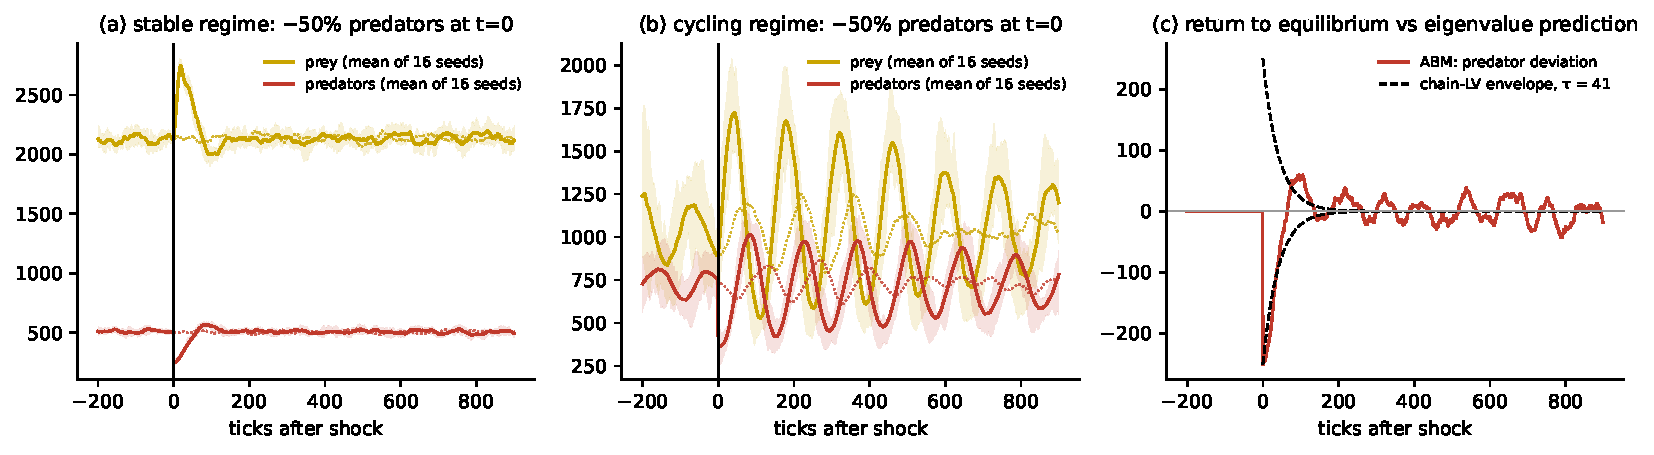
\includegraphics[width=\linewidth]{shocks.pdf}
\caption{Shock experiments averaged over many runs. (a) In the stable regime the populations swing back
to equilibrium in a few hundred ticks, with a decaying oscillation. (b) In the cycling regime the shock
just shifts the timing of the cycles. (c) The size of the deviation shrinks roughly like an
exponential envelope; its time constant can be predicted from a mathematical model (Section~\ref{sec:models}).}
\label{fig:shocks}
\end{figure}

A stable system that returns with decaying swings is called \textbf{underdamped} --- the same word you will meet
for a car suspension or a control loop. The time it takes for the swings to shrink by a factor $e\approx2.7$ is
the \textbf{time constant} $\tau$.

\begin{think}
Is there a shock big enough that the system does \emph{not} come back? Try \btn{$-50\%$ prey} three times in
quick succession. A stable equilibrium usually has a limited \emph{basin of attraction}: small pushes are
corrected, very large ones can tip the system somewhere else (e.g.\ extinction).
\end{think}

%=====================================================================
\section{Oscillations and delays}
%=====================================================================
Predator--prey systems are famous for \textbf{cycles}: prey boom, then predators boom, prey crash, predators
starve, and around it goes.

\begin{tryit}[: make it cycle]
Load \emph{Lotka-Volterra cycles} (identical to the stable case except that predators survive
30 ticks without food instead of 12). Run 2000 ticks.
\begin{enumerate}[nosep]
  \item Measure the \textbf{period}: ticks from one prey peak to the next.
  \item Which peaks first, prey or predators? By how much?
  \item Look at the phase portrait. Which way does the curve turn?
\end{enumerate}
\end{tryit}

\begin{idea}[: delay causes overshoot]
Why does a longer starvation time make the system oscillate? Predators react to food shortage only after a
\textbf{delay}: they keep eating even when prey are already scarce, so prey are pushed far below the
balance point, and then predators die all together. A balancing loop with a long delay overshoots ---
like a shower whose temperature responds slowly to the tap: you keep turning, overshoot, turn back,
overshoot again\ldots
\end{idea}

\begin{figure}[!htb]
\centering
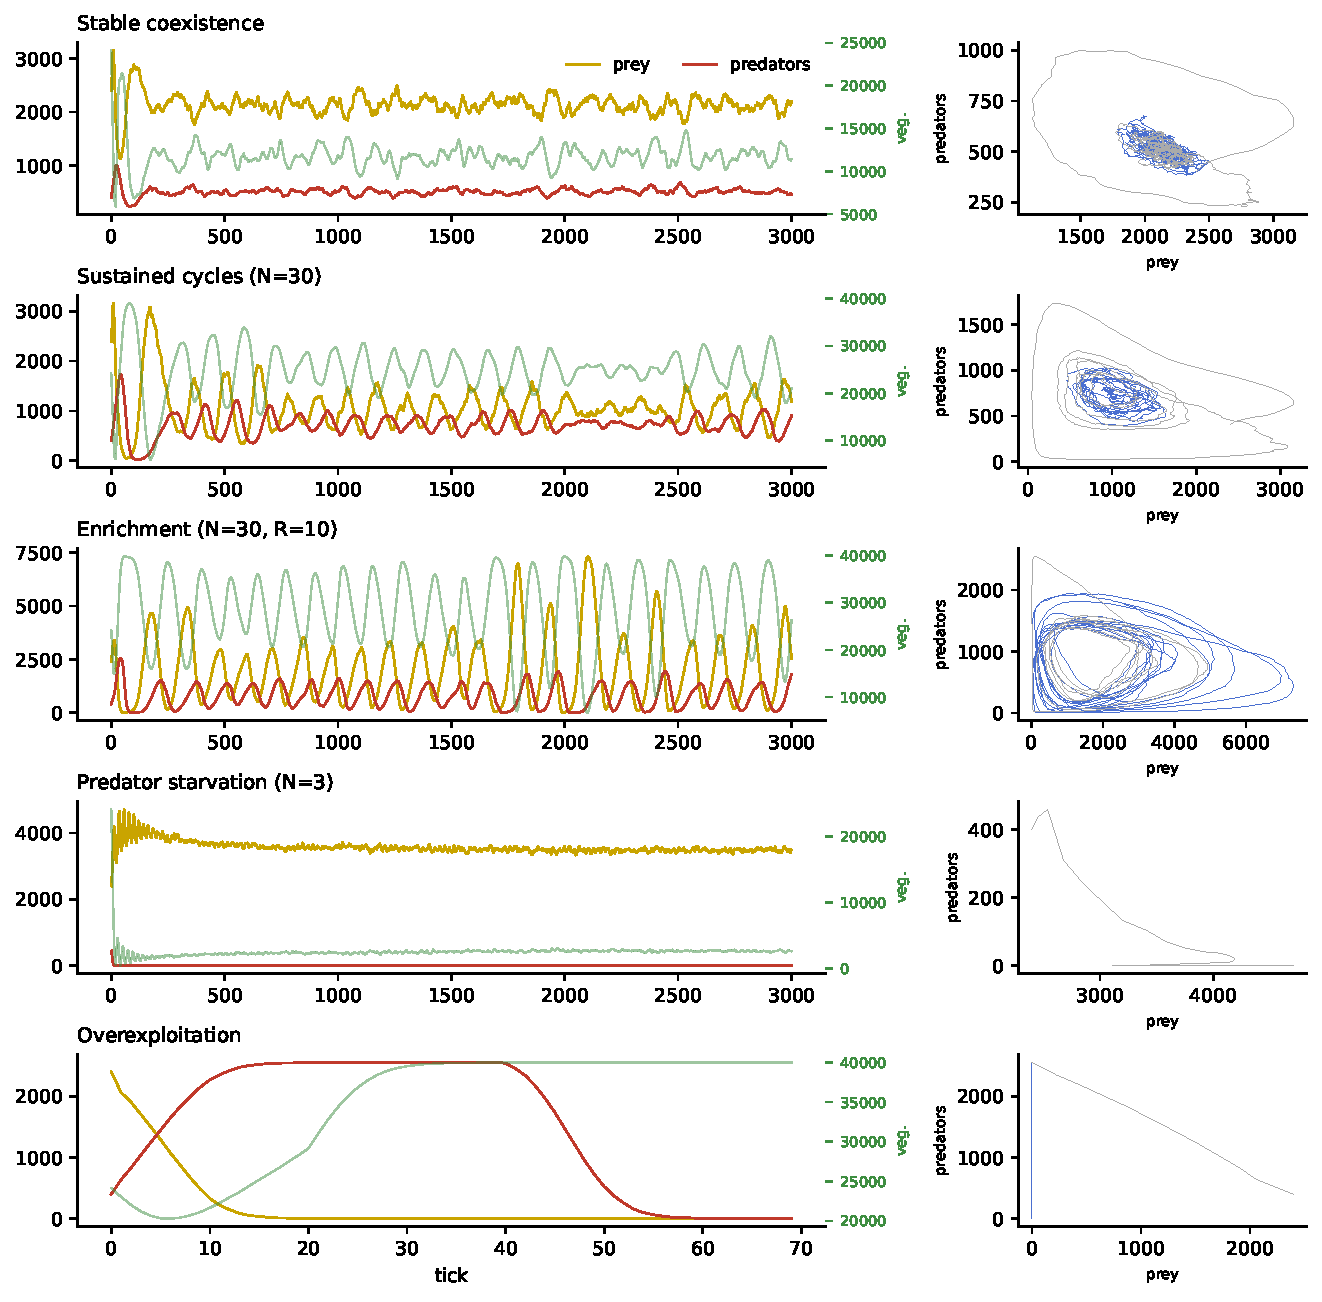
\includegraphics[width=\linewidth]{regimes.pdf}
\caption{Five regimes produced by the same rules with different parameters. Left: populations over time
(green, right axis: vegetation). Right: phase portraits, prey on the horizontal axis and predators on the
vertical (grey = start, blue = later). A cycle is a loop; a stable equilibrium is a small blob.}
\label{fig:regimes}
\end{figure}

\textbf{Reading a phase portrait.} Instead of plotting $x$ and $y$ against time, plot $y$ against $x$. Time
becomes a path. A point that stays put is an equilibrium; a closed loop is a cycle; an inward spiral is a
damped oscillation. In predator--prey systems the loop turns anticlockwise: prey grow (move right), then
predators grow (move up), then prey fall (left), then predators fall (down).

%=====================================================================
\section{Nonlinearity and tipping points}
%=====================================================================
\begin{idea}[: nonlinear means ``not proportional'']
In a \emph{linear} system, doubling the push doubles the response. Our ecosystem is \textbf{nonlinear}: a
small change can do almost nothing, or everything.
\end{idea}

\begin{tryit}[: the paradox of enrichment]
Compare \emph{Lotka-Volterra cycles} with \emph{Paradox of enrichment}, where vegetation grows back twice as
fast. More food should be good for everybody, right? Compare the size of the swings and the lowest
populations reached. Ecologists call this the \emph{paradox of enrichment} (Rosenzweig, 1971).
\end{tryit}

\begin{tryit}[: overexploitation]
Load \emph{Overexploitation}. Predators here are super-hunters. What happens to them in the end, and why?
A controller that is ``too good'' at its job can destroy the very thing it depends on.
\end{tryit}

%=====================================================================
\section{Models of the system}\label{sec:models}
%=====================================================================
In 1925--26 Alfred Lotka and Vito Volterra described predators and prey with two short equations. In words:
\begin{align*}
\text{change of prey per tick} &= \underbrace{a\,x}_{\text{births}} - \underbrace{b\,x\,y}_{\text{eaten}}\\
\text{change of predators per tick} &= \underbrace{c\,b\,x\,y}_{\text{births from food}} - \underbrace{g\,y}_{\text{deaths}}
\end{align*}
The term $b\,x\,y$ says: meetings between prey and predators are proportional to how many of each there are.
Setting both changes to zero (the equilibrium!) gives, with one line of algebra,
\[ x^\ast = \frac{g}{c\,b}, \qquad y^\ast = \frac{a}{b}, \]
which is the ``surprising consequence'' of Section~4: prey equilibrium depends only on predator numbers
$g, c, b$.

\begin{tryit}[: model versus simulation]
Run \emph{Lotka-Volterra cycles} for ~1500 ticks, then in the bottom panel choose a model and press \btn{Fit}.
The program measures births, deaths and kills in the simulation, estimates $a,b,c,g$, and draws the model's
prediction (dashed) on top of the simulation (solid). Try the different models in the menu.
\begin{enumerate}[nosep]
  \item Does the model get the \emph{average} populations right?
  \item Does it get the \emph{wobbles} right? The period?
  \item Choose \emph{Mean-field of rules}: a model built from the rules with no fitting at all, that ignores
        where animals are. How does it compare?
\end{enumerate}
\end{tryit}

\begin{idea}[: all models are wrong, some are useful]
The equations get the averages remarkably right, but they predict that the swings die out, while the
simulation keeps wobbling: random births and deaths keep ``kicking'' a system that, on its own, would settle.
The model also ignores \emph{space}: in the simulation predators eat the prey around them and must then
travel, which slows predation down by a factor of about three compared with a well-mixed world, and makes
the ecosystem much more stable. Choosing what to leave out of a model is the central skill of a
systems engineer.
\end{idea}

%=====================================================================
\section{Control: steering the ecosystem}\label{sec:control}
%=====================================================================
So far we only watched. Now we \emph{act}. Our actuator is \textbf{harvesting}: removing animals each tick
(think of fishing or culling). In control language:

\begin{center}
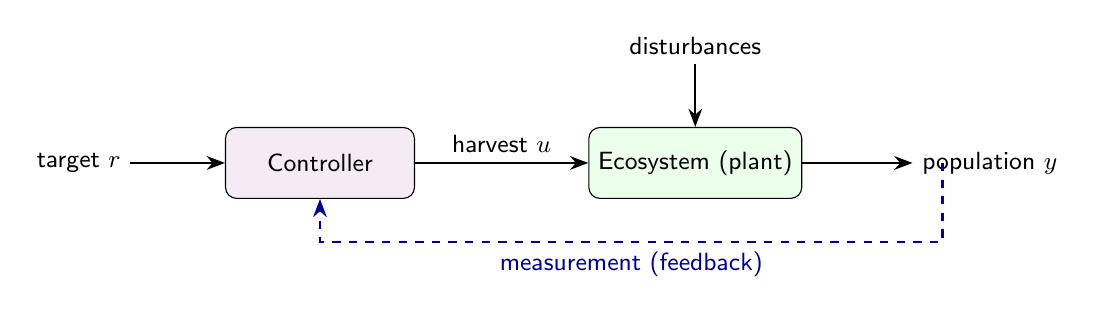
\begin{tikzpicture}[>=Stealth, node distance=1.6cm, every node/.style={font=\small\sffamily}]
  \node[draw, rounded corners, minimum width=2.4cm, minimum height=0.9cm, fill=violet!8] (C) {Controller};
  \node[draw, rounded corners, minimum width=2.4cm, minimum height=0.9cm, fill=green!8, right=2.2cm of C] (P) {Ecosystem (plant)};
  \node[left=1.2cm of C] (R) {target $r$};
  \node[right=1.4cm of P] (Y) {population $y$};
  \node[above=0.8cm of P] (D) {disturbances};
  \draw[->, thick] (R) -- (C);
  \draw[->, thick] (C) -- node[above] {harvest $u$} (P);
  \draw[->, thick] (P) -- (Y);
  \draw[->, thick] (D) -- (P);
  \draw[->, thick, blue!60!black, dashed] (Y) ++(-0.6,0) |- ++(0,-1.0) -| node[pos=0.25, below] {measurement (feedback)} (C.south);
\end{tikzpicture}
\end{center}

The \textbf{Control} group of parameters (bottom of the left panel) offers three controllers:

\begin{description}[nosep]
  \item[constant effort] remove a fixed \emph{fraction} of the population each tick (open loop);
  \item[constant quota] remove a fixed \emph{number} of animals each tick (open loop);
  \item[feedback (P-control)] measure the population $y$ and remove $K_p\,(y - r)$ animals each tick when
        $y$ is above the target $r$ (closed loop).
\end{description}
\param{harvest\_species} selects prey, predators or both, and \param{harvest\_start} the tick at which the
controller switches on, so that you can see the system before and after.

\begin{tryit}[: open loop -- quota versus effort]
Start from \emph{Stable coexistence}, harvest prey, \param{harvest\_start} = 500.
\begin{enumerate}[nosep]
  \item Constant quota of 20 prey per tick. Then 60. Then 80. What happens?
  \item Constant effort of 0.01, 0.03, 0.06. Compare.
\end{enumerate}
Which strategy is more dangerous, and why? (Hint: what does each one do when the population is already low?)
\end{tryit}

\begin{figure}[!htb]
\centering
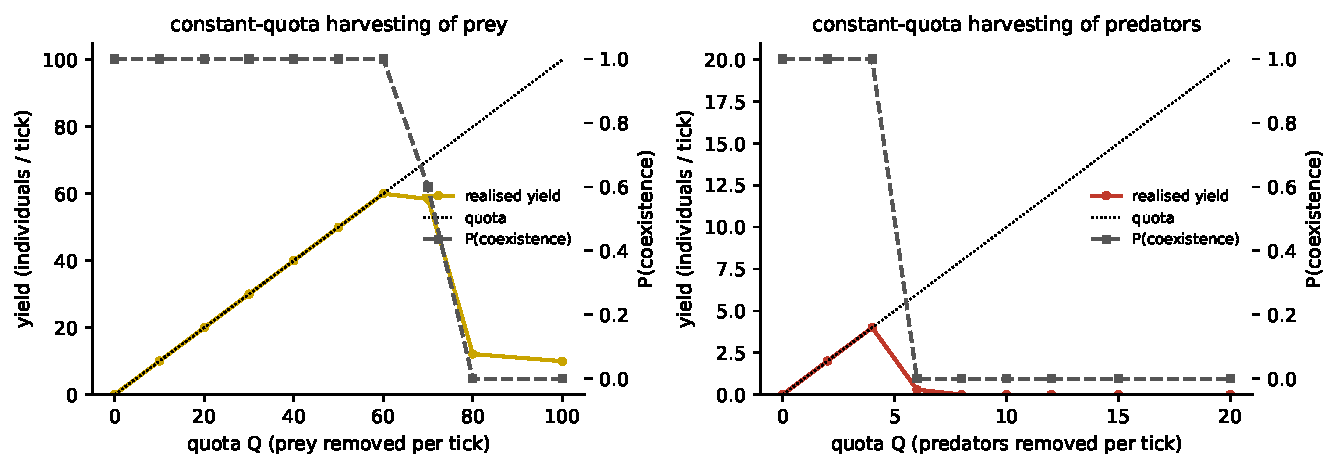
\includegraphics[width=0.9\linewidth]{harvest_quota.pdf}
\caption{Constant-quota harvesting: up to a threshold the yield equals the quota and both species survive;
just beyond it the prey population collapses and so does the ecosystem (grey: probability of coexistence).}
\label{fig:quota}
\end{figure}

\begin{control}[: why the quota tips over]
A quota is \emph{blind}: it takes the same number whether there are 3000 prey or 30. When prey are scarce it
takes a larger and larger \emph{fraction} of them --- a reinforcing loop towards extinction. Constant effort
takes a fixed fraction, so it automatically takes less when the population is low: it has a built-in
balancing loop. Real fisheries learned this lesson the hard way.
\end{control}

\begin{tryit}[: closed loop -- taming the cycles]
Load \emph{Lotka-Volterra cycles}. Set \emph{feedback} control on predators with target 400 and
\param{harvest\_start} = 1500. Try gains $K_p = 0.02,\ 0.2,\ 1$. Observe:
\begin{enumerate}[nosep]
  \item Do the cycles shrink after the controller switches on?
  \item Does the predator population sit exactly on the target?
  \item What does the controller do when predators are \emph{below} the target?
\end{enumerate}
\end{tryit}

\begin{figure}[!htb]
\centering
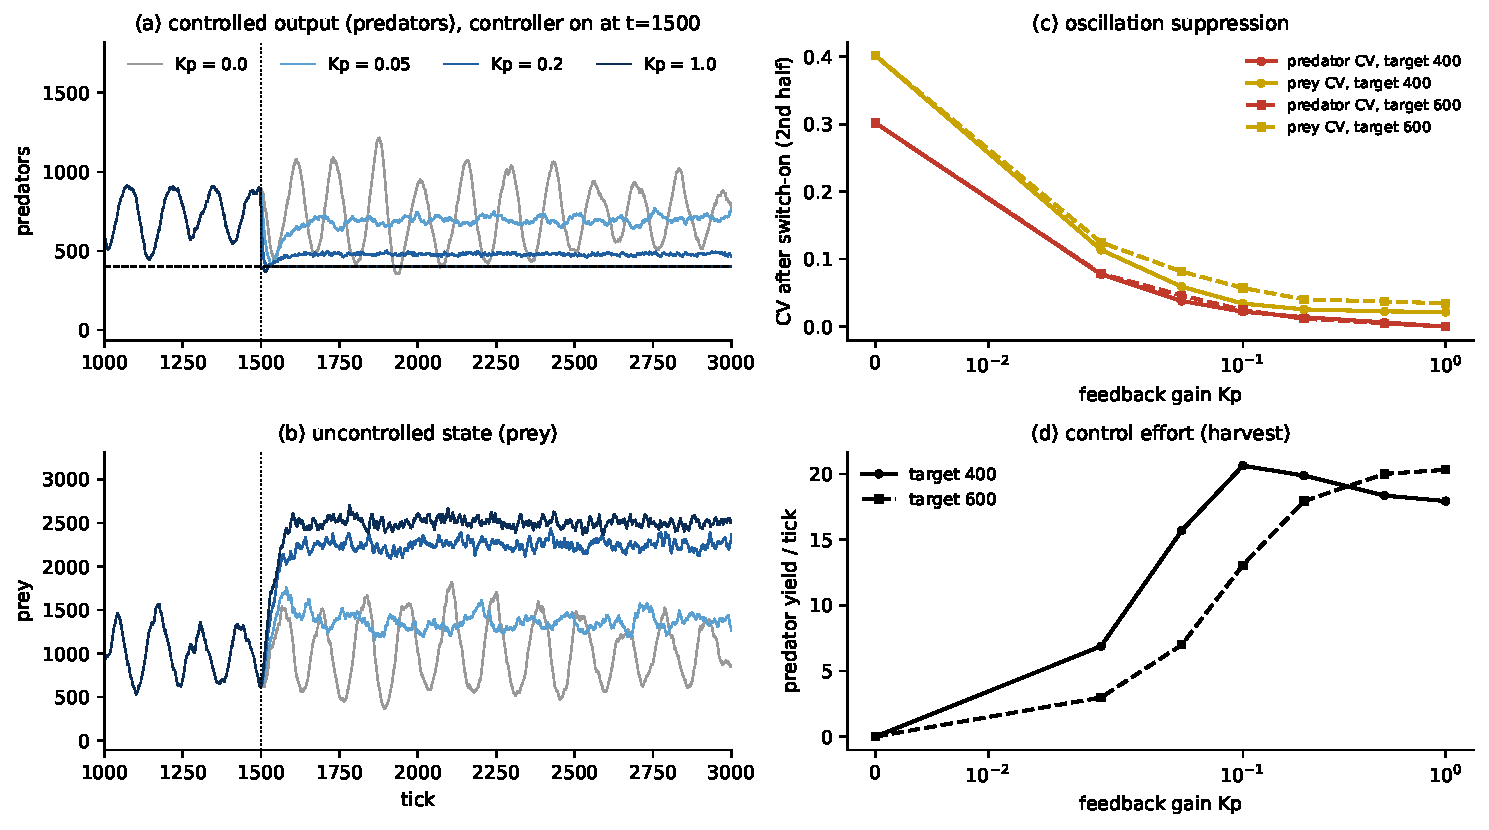
\includegraphics[width=\linewidth]{feedback.pdf}
\caption{Feedback control of predators in the cycling regime (switched on at $t=1500$). Higher gains cap the
predator peaks and the prey cycles shrink too, because the balancing loop through the predators is no longer
delayed. (c) Oscillation size versus gain, (d) the harvest the controller has to take.}
\label{fig:feedback}
\end{figure}

\begin{control}[: what you just discovered]
\begin{itemize}[nosep]
  \item \textbf{Feedback beats open loop} at rejecting disturbances: the controller reacts to what actually happens.
  \item \textbf{Actuator limits}: harvesting can only \emph{remove} animals. When the population is below target
        the controller can do nothing --- the actuator \emph{saturates}. Real actuators (motors, valves, heaters) always have limits.
  \item \textbf{Steady-state error}: a proportional controller only acts when there is an error, so the
        population hovers \emph{above} the target rather than on it.
  \item \textbf{Gain trade-off}: a small gain barely helps; a large one acts hard and takes a lot of harvest.
\end{itemize}
\end{control}

%=====================================================================
\section{Letting the computer search: optimisation}\label{sec:opt}
%=====================================================================
With 20+ parameters, trying combinations by hand is hopeless. The \textbf{Command Center} runs a
\textbf{genetic algorithm}: each candidate parameter set is a ``DNA''; many candidates are simulated, scored by
a \textbf{fitness} function, and the best are combined and mutated to form the next generation.

\begin{tryit}[: run an optimisation]
Open the Command Center. Choose the objective \emph{coexistence}, population 16, generations 8, ticks 800,
grid size 60, and untick every gene except \param{predator\_starve\_time}, \param{predator\_repro\_prob} and
\param{prey\_repro\_prob}. (A run this size takes a few minutes.) Press \btn{Start run} and watch the fitness chart. When it finishes, open the best
parameter set in the simulator. Is it really a robust ecosystem?
\end{tryit}

\begin{think}[: you get what you measure]
In our first large optimisation, the computer ``discovered'' that the easiest way to make both species survive
was to make predators that never reproduce and never die of old age --- a handful of immortal predators
living forever among a sea of prey. It satisfied the fitness function perfectly and was ecologically
meaningless. We fixed it by giving animals a finite lifespan and requiring both species to keep reproducing.
In control and optimisation, \emph{writing the right objective} is the hardest and most important step.
\end{think}

%=====================================================================
\section{Summary}
%=====================================================================
\begin{center}
\begin{tabular}{p{3.4cm}p{6.2cm}p{5cm}}
\toprule
\textbf{Concept} & \textbf{In the ecosystem} & \textbf{In engineering} \\
\midrule
State & prey, predators, vegetation & position \& speed of a car \\
Feedback loop & predators limit prey & thermostat \\
Equilibrium & births = deaths & room at set temperature \\
Stability & returns after a shock & suspension after a bump \\
Delay & predators starve slowly & slow shower tap \\
Oscillation & boom-and-bust cycles & under-damped motor \\
Nonlinearity & enrichment destabilises & saturating amplifier \\
Model & Lotka--Volterra equations & transfer function \\
Open-loop control & fixed quota / effort & toaster timer \\
Closed-loop control & harvest $\propto$ (population $-$ target) & cruise control \\
Optimisation & genetic algorithm & controller tuning \\
\bottomrule
\end{tabular}
\end{center}

%=====================================================================
\section*{Exercises}
\addcontentsline{toc}{section}{Exercises}
%=====================================================================
\begin{enumerate}[label=\textbf{E\arabic*.}]
  \item \textbf{Draw your own loop diagram} for a room with a heater controlled by a thermostat. Identify the
        balancing loop. Where would a delay come from?
  \item In \emph{Stable coexistence}, change \param{predator\_starve\_time} in steps 8, 12, 16, 20, 25, 30.
        For each, note whether the system is steady or cycling. At roughly which value does the behaviour change?
  \item Measure the time constant of the return after a $-50\%$ predator shock (time for the deviation to
        drop to about one third). Do it twice with different seeds. Why are the answers different?
  \item Make the grid smaller (\param{width} = \param{height} = 50) in \emph{Lotka-Volterra cycles}. Run five seeds.
        How often does an ecosystem collapse? Explain using the idea of random ``kicks''.
  \item Find the largest constant quota of prey that the stable ecosystem tolerates for 3000 ticks.
        Then find the effort that gives the same average yield. Compare how close each is to collapse.
  \item With feedback control on predators, plot (on paper) the average predator population against the gain
        $K_p$ for target 400. Why is it always above 400?
  \item Use the Command Center objective \emph{yield} with genes \param{harvest\_setpoint} and
        \param{harvest\_gain} (fix \param{harvest\_mode}=3 and \param{harvest\_species}=1). What controller does the
        computer find? Is it a sensible design?
\end{enumerate}

\subsection*{Hints}
\textbf{E2}: there is no sharp switch --- the wobbles grow steadily with $N$ (in our runs the prey CV goes from
about 0.06 at $N=12$ to 0.36 at $N=30$); below about $N=10$ predators go extinct and from about $N=50$ they
eat themselves out of food. \textbf{E3}: randomness --- each run is one sample of a noisy system; averaging many runs (as in
Fig.~\ref{fig:shocks}) gives a clean answer. \textbf{E4}: in a small world the random fluctuations are large
compared with the populations, so a trough can hit zero (in our runs a $40\times40$ cycling world never
survived 3000 ticks, $100\times100$ survived 4 times in 5, and $140\times140$ or larger always). \textbf{E5}: in our runs a quota of 60 prey/tick was tolerated and 70 already killed 2 of 5 ecosystems;
the quota fails abruptly, effort degrades gracefully. \textbf{E6}: a proportional controller needs an error to act.

\vfill
{\small\textit{The Lotka simulator, the experiments behind every figure and the companion research paper are
available at \url{https://github.com/hhpmacedo/lotka}.}}

\medskip
{\small\textit{How this guide was made.} This guide, the simulator and the experiments were produced by AI agents
(Hermes Agent running Anthropic's Claude models) under the direction of the author, and have not yet been
independently reviewed by the author. The project was inspired by an earlier university project on
predator--prey dynamics carried out with two university colleagues, who were not involved in this work.}
\end{document}
